\section{Software BMS}
Since the assignment was to understand the BMS, researching the system was initiated. When the group felt comfortable with the inputs and outputs of the system, small tests were executed to see if the BMS still worked as promised. The results of the tests were that the temperature and the cell voltages measurements worked as expected, but the CAN-communication did not. The test of the software can be seen on figure\vref{fig:SOFTWARE_REPORT_BMS}.\\

\begin{figure}[H]
	\centering
	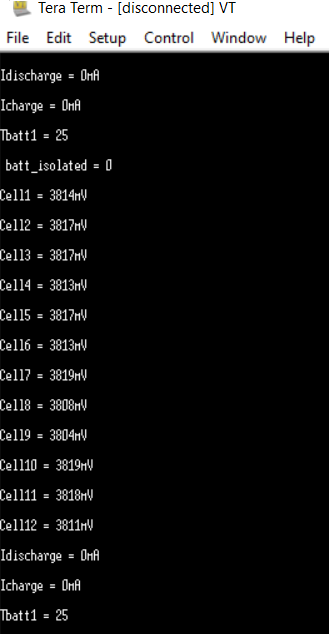
\includegraphics[width=0.4\linewidth]{SubPages/Images/BMS_teraterm_test.PNG}
	\caption{Test of the BMS software}
	\label{fig:SOFTWARE_REPORT_BMS}
\end{figure}

After trying to fix the CAN-communication, tests were executed. Here it was found out that the software for the Battery Management System that was given was the outdated 2013 version, which only works for a 6 celled battery. The 2014 version that was used with 12 cells was found in the end. There was no documentation for the software, so the group has reverse engineered the software to document the changes made in 2014, see the documentation\cite{AU2}(Section 5.4).\\
The CAN-communication could not be tested because of hardware problems, but the CAN-communication software must work because this was tested in the BMS 2013 Documentation\cite{BMSDocumentation}(Section 4.2.2 Page 91), and the functionality should be exactly the same.

The software is fully implemented and documented by Jonas Nyborg, the author of the BMS 2013 documentation\cite{BMSDocumentation}(Section 3.2). The only software function that is not documented is the CalculateSOC() function, which now has been documented\cite{AU2}(Section 5.4). Apart from that, not many significant changes have been made except for some changes to configurable definitions and the addition of the addresses to the Analog Front End Extension Module. These changes have been made in 2014 because the voltage level was doubled from 22.2V nominal to 44.4V nominal by adding an additional battery in series with the existing one. This also makes the Analog Front End Extension Module a necessity, and therefore addresses to this unit had to be added in the software, which also is documented\cite{AU2}(Section 5.4).   